\setcounter{page}{1}
\chapter{Introduction}
\label{intro}

As the title of this thesis suggests its background is twofold. On one hand it is founded on the theory of diffusion controlled reaction rates, on the other hand it is based on transition rate theory over fluctuating barriers. \\

\section{Transition Rate Theory} 

The subject of transition rate theory has been studied empirically even since the mid 18th century by Van't Hoff \cite{hoff1884} and Arrhenius \cite{arrhenius1889} but not before 1940 it became a thorough theoretical foundation when Kramers published his celebrated paper on ``Brownian Motion in a Field of Force and the Diffusion Model of Chemical Reactions'' \cite{Kramers1940}.  He described the escape from a metastable state as a noise assisted reaction and derived the well known Kramers reaction rate from the strong friction limit of the description of Brownian motion dynamics in phase space in presence of a nonlinear potential field.\vspace{- .5 cm} \par

\begin{minipage}[t]{0.62 \textwidth}
    \begin{figure}[H]
        \caption{Sketch of the system investigated in Doering\&Gadouas 1992 paper \cite{Doering1992} on Resonant Activation.  Two states between reflecting walls at $L$ and $-L$ are separated by a piecewise linear potential. The Potential that fluctuates between states of different height $E_+$ and $E_-$ subject to symmetric dichotomous noise with rate $\gamma$. Thermally activated particles that cross the barrier from one side to the other exhibit a minimum in mean first passage time depending on the rate of barrier fluctuations.\label{Gadoua}}
    \end{figure}
\end{minipage}\begin{minipage}[t]{0.38 \textwidth}
    \begin{figure}[H]
         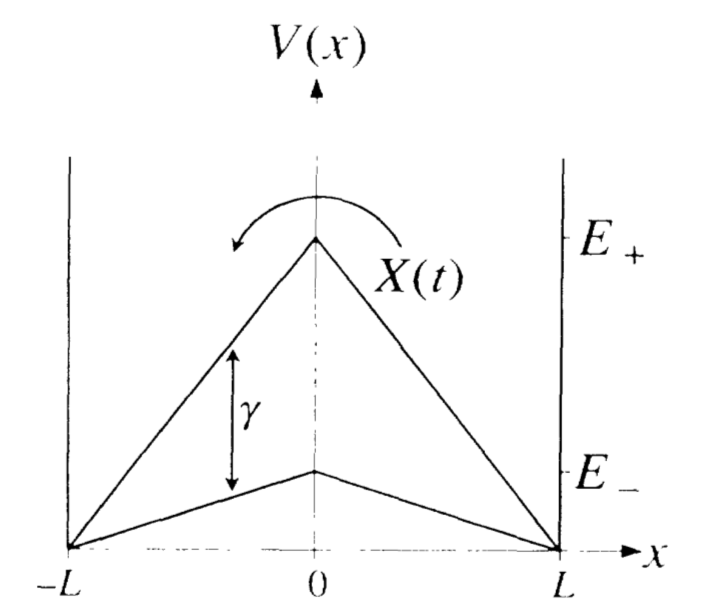
\includegraphics[width = 1 \textwidth]{plots/Gadoua.png}
    \end{figure}
\end{minipage}
\vspace{.3 cm}\\
Building up on Kramers results Doering and Gadoua \cite{Doering1992} were the first ones to investigate the case when the potential defining the metastable state in an escape problem is not constant but subject to fluctuations. Their setup consisted of a piecewise linear barrier between two reflecting walls that fluctuates between two distinct states in hight (see figure \ref{Gadoua}) as a Markov process with rate $\gamma$. They discovered an effect that they called \emph{resonant activation} that describes a local minimum in mean first passage times depending on the barrier fluctuation rate emerging from the interplay of the timescales of barrier crossing and barrier fluctuations. \\
In the following the effect has drawn signifficant interest of the community and has been thoroughly studied for several classes of potentials and a variety of processes describing the potential fluctuations \cite{Zurcher1993, Pechukas1994, Reimann1995, Reimann1995a}. The progress on the toppic has been nicely reviewed by Peter Reimann and Peter H\"{a}nggi in 1997 \cite{Reimann1997}

\section{Diffusion Controlled Reactions}
Reaction rate theory has been studied in physics, chemistry and biology since the early 19th century. All latter inquiries on the topic are founded on the pioneering work of Marian von Smoluchowski from 1916 and 1917 who held a series of talks \cite{Smoluchowski1916} describing the motion of Brownian particles in solution and used it to describe the coagulation of gold particles \cite{Smoluchowski1917a}. Thereby he obtain the famous Smoluchowski reaction rate of ideal Brownian particles of radius $R_p$ being absorbed in a spherical sink of radius $R_s$:\\
\begin{equation}
    K_S = 4 \pi D R_s \rho_0 \nonumber
    \label{Ksintro}
\end{equation}
where $D = D_p + D_s$ is the relative bulk diffusion constant, $\rho_0$ the bulk density of the Brownian particles and $R = R_p + R_s$ is the encounter distance. This result is valid for noninteracting, spherical and chemically isotropic reactants in ideal infinitely diluted solution. \\ 
Since these conditions strongly restricts the applicability of this general result to real world problems, the theory of diffusion controlled reactions has been widely extended in the course of the 19th century.\\
In the 1940s Debye \cite{Debye1942} extended this basic model to include inter particle interactions when he investigated the rate for diffusion limited reactions between charged particles in solution. Thereby he obtained the so called Smoluchowski Debye reaction rate:
\begin{equation}
    K_D = \rho_0\left\{\int_{R_s}^{\infty} \frac{\exp \left[ \frac{U(r')}{K_B T}\right]}{4 \pi D(r') r'^2} \rm d r' \right\}^{-1} \nonumber \nonumber
    \label{Kdintro}
\end{equation}
where $D(r)$ is the (not necessarily) spatially dependent diffusion profile, $U(r)$ is the interaction potential, $\rho_0$ is the bulk density of the particles and $R_s$ is the radius of the sink. \\
This approach is widely applied in i.e. heterogeneous catalysis, polymer chain growth kinetics, colloid or crystal growth and enzyme ligand binding. However, in most if these applications the reaction that takes place on encounter of the different diffusing components is not ideal but subject to a specific rate $K_A$ such that the process is governed by a kinetic rate $K_D$ arising from mass transport by diffusion and an interaction rate $K_A$ that is given by the particular reaction between the reactants. In this case the effective rate of the reaction turns out to be given by:
\begin{equation}
    K_{eff} = \frac{K_D K_A}{K_D + K_A}
    \label{KeffIntro}
\end{equation}
This expression serves neatly to explain the term \emph{diffusion controlled} reactions. Depending on the ration of $K_A$ and $K_D$ the process is either limited the reaction ($K_A \gg K_D$) or by mass transport ($K_A \ll K_D$) where the first case is called reaction controlled and the latter is called diffusion controlled. \\

To further extend the applicability of diffusion controlled reaction theory a variety of effects arising from finite densities and particle interactions have been taken into account. There are corrections due to hydrodynamic interaction between mutually approaching particles \cite{Friedman1966, Wolyes1976}, corrections due to combined hydrodynamic and hard sphere interaction for dilute but finite substrate concentration \cite{Dzubiella2005} as well as effects arising from crowding when substrate particles that are approximated as hard spheres occupy up to 30 -40 of the available volume \cite{Dorsaz2010}. Other generalizations include situations where there are multiple sinks competing for the substrate \cite{Reck1968a, Reck1968b} or setups where the reaction at the sink is limited to a certain reactive patch that covers only a fraction of its surface \cite{schmitz1972role, schurr1976, shoup1981diffusion, shoup1982role}. \\
Most of these effects have in common that they result in a spatially dependent or non isotropic diffusion profiles or tensors  or that they can be mapped to potentials of mean force describing the interaction between the species involved.
\newpage
\section{The Importance of Fluctuations}

In the 1880s Szabo et. al. \cite{Szabo1982} further extended the concept of diffusion controlled reactions to describe gating mechanisms. Motivated by the observation from biology namely that the rate of oxygen binding by hemoglobin is about an order of magnitude slower than expected when the reaction were completely diffusion controlled,\vspace{-1 cm}  \\

\begin{minipage}[t]{0.62 \textwidth}
    \begin{figure}[H]
        \caption{Structure of Au-PNIPA Yolk-Shell Nanoparticles studied by S. Wu, J. Dzubiella et al. The system consists of an Au nanoparticle of radius $R_0$ surrounded by a polymer shell with inner and outer radii $R_1$ and $R_2$ respectively. Reactants need a free energy $\Delta G$ to penetrate the polymer shell which therefore acts as a potential barrier. At the polymers lower critical solution temperature undergoes fluctuations between a hydrophilic and a hydrophobic state state resulting in different free energy barriers.}\label{PNIPA}
    \end{figure}
\end{minipage}\begin{minipage}[t]{0.38 \textwidth}
    \begin{figure}[H]
         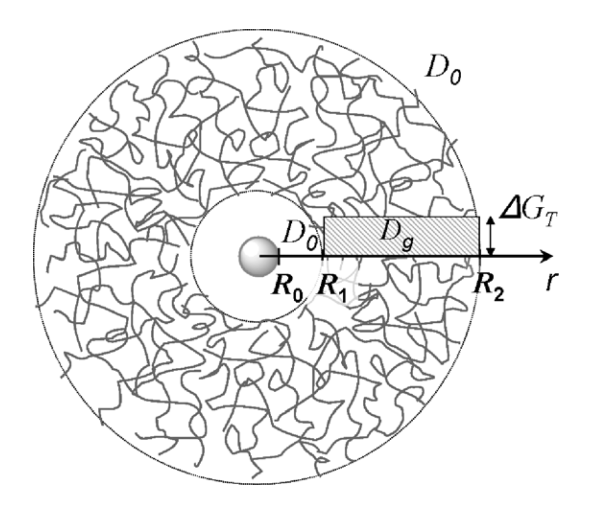
\includegraphics[width = 1.1 \textwidth]{plots/PNIPA.png}
    \end{figure}
\end{minipage}
\vspace{0.3 cm} \\
they reasoned that the binding cite of the protein was blocked by certain side chains such that the oxygen could not bind if they were in their equilibrium position. Due to the dynamic nature of proteins these chains were thought to not be fixed but rather fluctuate between states where they inhibit the oxygen from binding and states where oxygen binding is possible thus acting as a gate for the reaction. \par
To translate this behavior to the picture of Brownian particles and an absorbing sink, the sink was no longer considered to be ideal but was taken to fluctuate between different states of surface reactivity. The analytic work in this thesis is to some extend inspired by the methods they employed to treat the problem of diffusing particles switching between states with different boundary conditions representing the gated nature of the sink. \\

Now in many problems it is not (only) the reactivity of a binding site that is fluctuating but the interaction between in terms of forces between the reactants involved. One recent example are the thermosensitive yolk-shell nanoparticles studied by Shuang Wu, Joachim Dzubiella et al. \cite{Wu2012a}. They consist of a reactive Au nanoparticle encapsulated in a thermosensitive polymer shell. The solvation free energy $G(r)$ within the polymer shell differs significantly from that in the bulk such that it represents a potential barrier that reactants have to overcome to get in contact with the catalytic core. As the polymer undergoes a phase transition between states of different salvation energy this barrier stochasically fluctuates between states of different hight. This results in nonlinearities in the Arrhenius plot of the reaction rate of the system that remain unexplained in detail so far.\\

Another interesting problem that involves reactions over fluctuating barriers is hydrophobic cavity-ligand binding. When P. Sethy et al. \cite{Setny2013} investigated on a system consisting of ligand binding to a hydrophobic pocket in presence of water they discovered that the pocket undergoes whet/dry transitions i.e. it stochastically switches between a state where it is filled with water and a state where it is depleted and empty. For both of these states it was possible to extract a potential of mean force for the pocket ligand interaction and effective friction profiles for the movement of the ligand approaching the pocket. The problem has been approached by numeric treatment of a composite Markov model for a discrete reaction coordinate representing the state of the pocket and a continuous coordinate for the ligand pocket distance by J. Mondal et al. \cite{Mondal2013} but still lacks a thorough analytic treatment. \\

In fact similar effects of fluctuating interaction between reactants or adsorbants coupling to diffusional motion are common in polymer and soft matter physics since pH or temperature triggered phase transitions of polymer networks such as hydrogels \cite{Cai2011} are widely employed in i.e. carrier systems for targeted drug delivery \cite{yoshida1995comb, gupta2002hydrogels}, homeostatic, self regulating materials \cite{He2012} or to trigger microfluidic channels \cite{Beebe2000}. \\

\comment{That one I'm pretty uncertain about since I don not have any idea about relative timescales of spatial conformation and protonation of macromolecules. Might be that they are well separable, might be that under certain conditions they are not. Any ideas?}
One more not so obvious application might be protein folding. The pH controlled self assembly of i.e. spider silk proteins \cite{Askarieh2010} is supposed to be dominated by the protonation of a certain domain of the protein leading to conformational changes that favor fiber formation \cite{Gaines2010}. The protonation of protein cites is a discrete process and therefore subject to thermal fluctuations. If self assembly of the protein is described as a random walk on a free energy landscape representing the possible protein conformations \cite{frauenfelder1991, Onuchic1997, Rathore2002} this energy landscape is strongly influenced by the charge conformation of the protein and therefore fluctuating due to the stochastic nature of protonation. Consequently the problem is that of a random walk on a fluctuating energy landscape with one absorbing state representing the final conformation of the protein. \\

To sum up: the transition over fluctuating barriers is well understod for escape problems but although there is a variety of applications it has not yet been thoroughly approached in the context of diffusion controlled reaction rate theory.
\newpage
\section{A Minimal Model for Reaction Rates over Fluctuating Barriers}
\label{mini_model}
As a feasible approach to the problem of diffusion controlled reaction over fluctuating barriers this thesis will study a spherical sink that is surrounded by a step shaped potential barrier fluctuating in hight and embedded in a bath of Brownian particles as illustrated in figure \ref{introSketch}. The limits of very fast and very slow barrier fluctuations can easily be deduced in \par
\begin{wrapfigure}[18]{o}{0.44 \textwidth}
    \hspace{-2 cm}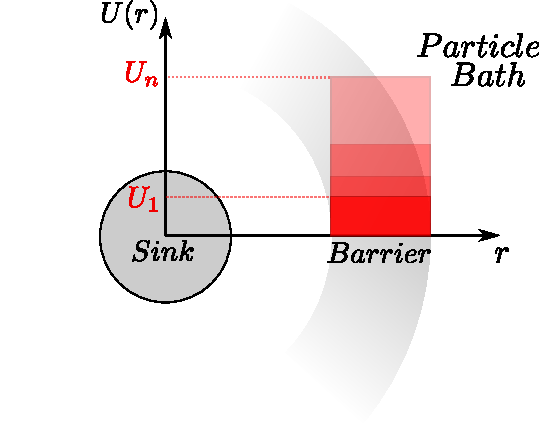
\includegraphics[width = 1.1 \textwidth]{plots/IntroSkizze.pdf}
    \caption{Sketch of system consisting of a spherical sink surrounded by a spherically symmetric step shaped barrier (indicated in \textcolor{red}{red}) embedded in a bath of Brownian particles.}
    \label{introSketch}
\end{wrapfigure}
analogy to the escape problem studied by Doering and Gadoua.
For barrier fluctuations that are fast compared to the diffusional relaxation of the Brownian particles it can be assumed that the particles move subject to a potential of mean force, such that the rate approaches that over an average barrier. For barrier fluctuations that are very slow compared to the diffusional relaxation of the particles the rate approaches the average of the rates over the different barrier configurations.
If it is not possible to separate the timescales of particle diffusion and barrier fluctuations more complex behavior arises. This behavior will be the main focus of this thesis. 
Other points of interest are the dependence of effects on the spherical geometry of the system and the connection to experiment and simulations where it is common practice to reduce complex systems to only their reaction coordinates which often leads to complex diffusivity profiles and non Markovian behavior.

\section{Thesis Outline}
To follow an educative approach chapter \ref{Short_Introduction_to_Stochastic_Processes} gives a short introduction to stochastic processes as far as it is helpful to supplement A) the examples from diffusion controlled reaction theory in section \ref{K_s} and \ref{The_Debye_Reaction_Rate} and B) the derivations made in section \ref{Reaction_Rates_over_Fluctuating_Barriers}. \\
Chapter \ref{Reaction_Rates_over_Fluctuating_Barriers} gives an analytical treatment of a system consisting of a spherical sink surrounded by a metastable step shaped potential barrier that is embedded by a bath of Brownian particles and derives an expression for the rate of encounters of these particles with the sink. \\
Chapter \ref{numeric_model} gives a short resume of the numerical methods in use. Chapter \ref{results} evaluates a simple example of the system described in chapter \ref{Reaction_Rates_over_Fluctuating_Barriers}. It analyzes the effects arising from coupling between diffusional relaxation and barrier fluctuations in terms of particle fluxes, gives a thorough study of all relevant parameters and finally tries to bridge the gap to experiments by interrogating on effects that arise from the reduction of the system to only the spatial coordinates through averaging over potential fluctuations. Chapter \ref{conclusion} sums up the results and gives an outlook on further work. \\

The keen reader may skip chapter \ref{Short_Introduction_to_Stochastic_Processes} and \ref{numeric_model} since they are basically a collection of relevant textbook knowledge and proceed directly with chapter \ref{Reaction_Rates_over_Fluctuating_Barriers} and \ref{results} which contain newly obtained results. 
